\documentclass[10pt]{article}
\usepackage[margin=1in]{geometry}
\usepackage[T1]{fontenc}
\usepackage{lmodern,amsmath,amssymb,amsthm,mathtools}
\usepackage{booktabs,array,graphicx,microtype}
\usepackage[colorlinks=true,allcolors=blue!50!black]{hyperref}
\usepackage{xcolor}
\newtheorem{theorem}{Theorem}[section]
\newtheorem{lemma}[theorem]{Lemma}
\newtheorem{corollary}[theorem]{Corollary}
\newtheorem{proposition}[theorem]{Proposition}
\newtheorem{assumption}[theorem]{Assumption}
\newtheorem{definition}[theorem]{Definition}
\title{COMET: Counterfactual Moment Auditing under\\Weak Overlap and Graph Dependence}
\author{Anonymous research draft}
\date{Local research revision, 15 November 2026}
\begin{document}
\maketitle

\begin{abstract}
Counterfactual moment auditing asks which subgroup and policy conclusions have
enough evidence under selective, dependent feedback. We study finite families
of signed moments under a heterogeneous fixed design, exact supported exposure
laws, valid residual moment envelopes, independent training information and a
sufficient global conditional dependency graph. Separating the known direct
term from a clipped weighted residual yields an explicit certificate for the
original moment: sharp clipping bias, graph-adjusted concentration and a range
term. Unequal row means and one connected graph are allowed. Query-specific
support and paired contrasts identify the relevant overlap and dependence
costs, while a scoped two-point subclass gives an evidence obstruction.

Completed synthetic studies distinguish coverage from decision value. Across
12,000 heterogeneous-graph logs, all 96 eligible primary comparisons cover the
complete query family in 1,000/1,000 trials per fixed comparison, yet all six
finite-moment cells have zero violation detections. Local questions avoid
irrelevant outside hubs and extreme weights; direct contrasts can certify a
risk reduction when subtraction of jointly certified levels cannot. In 4,000
independent discovery-to-selection trials, nonbaseline safe returns with
positive utility gain occur in 500/500 trials per moderate-overlap cell and
231--411/500 per weak-overlap cell, with no observed unsafe COMET return.
Baseline noninferiority is reported separately. The fully matched generic
construction is algebraically and empirically identical; eligible IID
DR empirical-Bernstein and Catoni comparisons can be narrower. The contribution
is a query-specific certification and evidence-cost analysis with explicit
decision consequences.
\end{abstract}

\section{Which counterfactual questions have enough evidence?}

A rare exposure can carry a large inverse-probability weight, and shared
randomness can make many observed rows convey less information than their count
suggests. These two difficulties interact with the question being asked.
A policy change supported on a small region should not automatically pay for
an unrelated rare exposure elsewhere; a subgroup contrast should not require
two imprecise policy levels when its signed residual cancels outside that
subgroup. The relevant object is therefore a family of explicit, supported
counterfactual moments together with their evidence requirements.

We formulate these questions conditional on an exogenous design. Rows can
have different conditional means and can form one connected dependency graph.
The graph is sufficient for the entire random score vector, with independence
between disjoint sets that have no crossing edge. This requirement is stronger
than a drawing of the application network, pairwise zero covariance, or a graph
inferred from one realized log. Independent random-source incidence provides
a constructive sufficient model.

The main construction separates the known direct prediction term from the
random weighted residual. It clips the residual at a threshold fixed before
certification outcomes and pays for both the resulting worst-case bias and
graph-adjusted fluctuations. The resulting interval covers the original
unclipped signed moment. The statistical ingredients are standard clipping
and concentration tools; graph-coloring concentration has a substantial prior
literature~\cite{janson2004}. We formulate and analyze how support, contrasts,
residual moments and a sufficient graph determine the evidence cost of an
auditing question. A generic truncated graph mean with fully matched
information is the same procedure; the contribution therefore concerns this
formulation and analysis, its limits and its decision consequences.

Independent construction followed by risk-controlled selection has clear
precedents. Learn then Test combines valid tests with familywise error control
to protect a returned set~\cite{angelopoulos2025ltt}; high-confidence policy
improvement separates candidate search from a held-out safety
test~\cite{thomas2015hcpi}. In the present model, this logic requires valid
certificates for heterogeneous signed moments under a sufficient conditional
graph. The analysis connects those certificates to support, residual moments,
paired comparisons and a scoped evidence-cost obstruction.

Three questions must be kept separate. First, are the assumptions sufficient
and the implementation consistent with the stated theorem? Second, is the
resulting interval informative for the given subgroup, overlap and graph?
Third, does it return a policy that is simultaneously safe and useful?
The historical confirmation study illustrates why coverage alone cannot answer
the latter two questions. The experiments evaluate these distinctions under
heterogeneous connected graphs and independent discovery. The completed
validity grid already shows that full-family coverage can coexist with zero
detection in every tested heavy-tail cell, while stronger bounded inference
can recover useful detection. Query-local ablations and a fully informed
equal comparator separate gains from relevant information from gains
attributable to a distinct statistical procedure.

\section{Certificates and query-specific evidence costs}
\label{sec:post-cstat-theory}

The object of inference is a fixed-design moment. The probability model permits
heterogeneous row means and one connected dependency graph; it does not require
independent repeated macro-blocks or equal block targets. We condition throughout
on a legitimate exogenous field $\mathcal D$, augmented only by training and
discovery information whose random sources are independent of certification.
A schema can check a declared source construction, but cannot establish the
absence of unrecorded common causes from a single realized log.

\paragraph{Signed moments and support.}
For coordinate $\theta$, let $c_\theta$ identify its response channel, and write
$Y_{u,\theta}$, $\mu_{us,\theta}$ and $\widehat\mu_{us,\theta}$ for the response,
identified exposure-specific mean and fixed nuisance fit. The finite exposure
law $e_{us}=\Pr(S_u=s\mid\mathcal D)$ is known exactly. Define
\begin{align}
 M_\theta
 &=a_\theta+\frac{1}{B_\theta}
     \sum_{u=1}^N\sum_s d_{us,\theta}\mu_{us,\theta},
 &B_\theta&=N\,\mathrm{normalizer}_\theta>0,
 \label{eq:post-target}\\
 D_\theta
 &=a_\theta+\frac{1}{B_\theta}
     \sum_{u,s}d_{us,\theta}\widehat\mu_{us,\theta},
 &R_{u,\theta}
 &=\frac{d_{uS_u,\theta}}{e_{uS_u}}
       (Y_{u,\theta}-\widehat\mu_{uS_u,\theta}).
 \label{eq:post-residual}
\end{align}
Here $a_\theta$, $B_\theta$ and the signed coefficients $d_{us,\theta}$ are
$\mathcal D$-measurable. A level query uses $d=hq$; a paired policy contrast
uses $d=h(q-q_0)$. A subgroup ratio uses its known positive design mass in
$\mathrm{normalizer}_\theta$; a zero-mass ratio is undefined. Every nonzero
coefficient requires $e_{us}>0$. Exact exposure probabilities identify the
counterfactual mean only together with the stated exposure sufficiency and
assignment assumptions. A policy interpretation additionally requires that
$q$ arise from a compatible joint assignment law.

Support is a property of the question. For bounded responses with exposure
law $e=(0,1/2,1/2)$, consider
$q_0=(1/5,3/10,1/2)$ and $q_1=(1/5,1/2,3/10)$.
Neither policy level is point identified when the first state's mean is
unknown. Their signed contrast has coefficient
$q_1-q_0=(0,1/5,-1/5)$ and uses only observed states. The common unsupported
contribution cancels. Every matched contrast-aware method receives this
same supported query.

\begin{assumption}[Conditional graph and residual envelopes]
\label{ass:post-core}
The desired exposure-specific means satisfy
$\mathbb E[Y_{u,\theta}\mid S_u=s,\mathcal D]=\mu_{us,\theta}$.
The entire row score/residual vector has a sufficient conditional dependency
graph $G$: disjoint vertex sets with no crossing edge are conditionally
independent given $\mathcal D$. For a declared $1<p\leq2$, known numbers
$b_{us,\theta}\geq0$ satisfy
\begin{equation}
 \mathbb E\!\left[
 |Y_{u,\theta}-\widehat\mu_{us,\theta}|^p
 \mid S_u=s,\mathcal D\right]\leq b_{us,\theta}^p.
 \label{eq:post-channel-envelope}
\end{equation}
The query family, all confidence allocations and all tuning choices are fixed
conditional on $\mathcal D$ before certification outcomes are examined.
\end{assumption}

A sufficient constructive graph connects every pair of rows sharing any
independent primitive source used in logging or in any retained response
channel. Its sufficiency follows from disjoint source collections, not from
observed correlations or a domain network alone. Let $A_\theta$ be the rows
whose residual is not identically zero by design. Use the induced graph
$G[A_\theta]$ and the smallest number $\chi_\theta$ among the available,
verified proper colorings. This is an available coloring count, rather than
a claim to compute the chromatic number. All source-induced edges between
retained rows remain present even when other rows are removed.

Set
\begin{equation}
 v_{u,\theta}
 =\sum_{s:e_{us}>0}|d_{us,\theta}|^p e_{us}^{1-p}b_{us,\theta}^p,
 \qquad
 c_p=\frac{(p-1)^{p-1}}{p^p}.
 \label{eq:post-v}
\end{equation}
These bound raw residual moments; a centered-noise moment cannot be substituted
without accounting for nuisance error. In bounded responses $Y\in[L,U]$, the
legal residual magnitude is $\max\{|L-\widehat\mu|,|U-\widehat\mu|\}$.
In particular, midpoint nuisance on $[0,1]$ gives magnitude $1/2$ for every
eligible comparison method.

\begin{theorem}[Heterogeneous conditional-graph residual certificate]
\label{thm:post-core}
Under Assumption~\ref{ass:post-core}, choose positive $\mathcal D$-measurable
thresholds $\tau_{u,\theta}$ on the active support and let
$T_\tau(x)=\operatorname{sign}(x)\min\{|x|,\tau\}$. For a coordinate budget
$\delta_\theta\in(0,1)$, put $t_\theta=\log(2/\delta_\theta)$ and define
\begin{align}
 \widehat M_\theta
 &=D_\theta+\frac{1}{B_\theta}
           \sum_{u\in A_\theta}T_{\tau_{u,\theta}}(R_{u,\theta}),
 \label{eq:post-estimator}\\
 r_\theta
 &=\frac{1}{B_\theta}\left[
 c_p\sum_{u\in A_\theta}v_{u,\theta}\tau_{u,\theta}^{1-p}
 +\sqrt{2\chi_\theta t_\theta
           \sum_{u\in A_\theta}v_{u,\theta}\tau_{u,\theta}^{2-p}}
 +\frac{2}{3}\chi_\theta t_\theta
                   \max_{u\in A_\theta}\tau_{u,\theta}\right].
 \label{eq:post-radius}
\end{align}
Then $\Pr(|\widehat M_\theta-M_\theta|>r_\theta\mid\mathcal D)
\leq\delta_\theta$. For a finite frozen family $\Theta$ with
$\sum_{\theta\in\Theta}\delta_\theta\leq\delta$, all coordinate intervals
cover simultaneously with conditional probability at least $1-\delta$.
If no random residual remains, its radius is zero and the known direct term
is retained.
\end{theorem}

The three terms in~\eqref{eq:post-radius} pay for clipping bias, graph-adjusted
fluctuation and bounded range, respectively. The target is the original
unclipped moment. Clipping without the first term targets a different object
unless a separate argument removes the bias. One threshold per query is the
special case $\tau_{u,\theta}=\tau_\theta$ used by the initial implementation.
The proof, including the graph MGF step, appears in
Appendix~\ref{app:post-proofs}.
Each family statement concerns one predeclared construction per coordinate,
including a design-only dispatch when used. It does not automatically give
joint coverage over all plotted methods and both nominal levels. Such a claim
would require allocating the total budget across method, level and query.

\begin{corollary}[Locality, design-only tuning and paired scaling]
\label{cor:post-locality}
Removing design-inactive rows leaves the estimand and direct term unchanged,
and permits the induced support graph in Theorem~\ref{thm:post-core}.
Thresholds and eligible certificate engines may be selected by minimizing a
proved radius over a predeclared design-only grid without an additional
outcome-search budget. For a signed contrast scaled by $\eta>0$, scaling its
thresholds by $\eta$ scales its signal and every radius component by $\eta$;
$\eta=0$ has zero random uncertainty. Small policy steps therefore do not by
themselves improve sign-certification power.
\end{corollary}

\paragraph{Sharp bounded comparisons.}
For known response bounds, let $[\ell_{u,\theta},u_{u,\theta}]$ be the actual
possible residual interval, taking extrema over every supported exposure, and
write $w_{u,\theta}=u_{u,\theta}-\ell_{u,\theta}$. With the same query, nuisance,
support, graph and coordinate budget, the untruncated estimator
$\widehat M^{\mathrm{mean}}_\theta=D_\theta+B_\theta^{-1}\sum_u R_{u,\theta}$
has graph Hoeffding and Bernstein radii
\begin{align}
 r_{H,\theta}
 &=\frac{1}{B_\theta}
       \sqrt{\frac{\chi_\theta t_\theta}{2}\sum_u w_{u,\theta}^2},
 \label{eq:post-hoeffding}\\
 r_{B,\theta}
 &=\frac{1}{B_\theta}\left[
       \sqrt{2\chi_\theta t_\theta\sum_u V_{u,\theta}}
       +\frac{\chi_\theta t_\theta}{3}\max_u w_{u,\theta}\right],
 \quad
 V_{u,\theta}=\min\left\{v^{(2)}_{u,\theta},
                               \frac{w_{u,\theta}^2}{4}\right\},
 \label{eq:post-bernstein}
\end{align}
where $v^{(2)}$ is the legal raw second-moment bound from the known bounded
response class. The same bounds and envelope information are supplied to all
matched methods. A generic bias-corrected truncated graph mean with the same
inputs and tuning is algebraically identical to the corresponding
configuration of~\eqref{eq:post-estimator}--\eqref{eq:post-radius}; equality is
a comparison result, not evidence of estimator superiority.

For the historical A design alone, $q=e=(1/2,1/2)$, midpoint nuisance and
reference $1/4$ give score $Y-1/4$. At $N=8192$, $m=1$, $\chi=1$ and
$\delta=.05$,
\begin{equation}
 r_H=\sqrt{\frac{\log 40}{2\cdot8192}}
       =0.015005043614373761,
 \qquad
 .0375>2r_H.
 \label{eq:post-A-fixture}
\end{equation}
This is a deterministic analytic comparison: on its coverage event the lower
bound for target $.2375$ exceeds threshold $.2$. It is not new measured power
and is not included in the old seventeen-test confirmation family.

\begin{proposition}[A scoped subgroup--overlap--dependence obstruction]
\label{prop:post-lower}
Let $g=N\pi$ be a positive integer divisible by $\chi$, set $n=g/\chi$, and
fix $\epsilon\in(0,1]$, $\nu>0$, $1<p\leq2$ and a mean-deviation cap $H>0$.
There is a supported, exactly known logging experiment on $n$ independent
$\chi$-row cliques, with exposure probability $\epsilon$ and unweighted
potential-response residual moment
$\mathbb E|Y(1)-b|^p\leq\nu^p$, for which every estimator of the normalized
subgroup mean has worst-case expected absolute error at least
\begin{equation}
 \frac12\min\left\{H,
 \nu\min\left(1,(2n\epsilon)^{-\frac{p-1}{p}}\right)\right\}.
 \label{eq:post-lower}
\end{equation}
The corresponding raw importance-weighted residual moment is at most
$\epsilon^{1-p}\nu^p$; $\nu$ is the response-residual scale, before
importance weighting. For the raw subgroup moment the bound is multiplied
by $\pi$. In its
unsaturated regime this gives normalized scale
$\nu(\chi/(N\pi\epsilon))^{(p-1)/p}$, up to the displayed constant.
It does not establish graph-by-graph sharpness or matching simultaneous
confidence logarithms. The construction and a non-sharp confidence-width
consequence are in Appendix~\ref{app:post-lower}.
\end{proposition}

A symmetric certificate with radius $r$ certifies a true threshold violation
on its coverage event whenever its true gap satisfies $\gamma>2r$.
This is a sufficient procedure-specific decision condition. The lower bound
is a separate necessary expected-risk obstruction on its stated subclass;
neither statement turns a conservative radius map into a sharp information
limit for every design.

\begin{corollary}[Independent discovery and certified finite selection]
\label{cor:post-selection}
A finite family selected using independent discovery sources may be included
in $\mathcal D$. The simultaneous family must contain every risk coordinate
and utility contrast actually used by selection. On its coverage event,
returning only a candidate whose risk upper bounds meet the task constraints,
whose exact design service/capacity meet their bounds, and whose utility lower
contrast meets the declared usefulness requirement is safe and useful in that
fixed-design sense. In particular,
$\Pr(\mathrm{return}\ \mathrm{and}\ \mathrm{unsafe})\leq\delta$.
There is no corresponding automatic $\delta$ guarantee for
$\Pr(\mathrm{unsafe}\mid\mathrm{return})$ and no theorem here guaranteeing
a positive return rate.
\end{corollary}

\begin{corollary}[Affine mixtures on the simultaneous event]
\label{cor:post-mixtures}
Let $Q_j$ be compatible base joint policies with fixed auditors and normalizers.
For nonnegative weights summing to one, $Q_w=\sum_jw_jQ_j$ is a valid joint
mixture. Simultaneous base intervals propagate to
$[\sum_jw_jL_j,\sum_jw_jU_j]$ for each affine moment, even for weights selected
after seeing the certificates. This is linear propagation of certified base
quantities, not permission to recompute a nonlinear clipped estimator at an
outcome-selected mixture. Nonlinear metrics or moving denominators require
separate analysis.
\end{corollary}

All statements above concern real arithmetic under declared assumptions.
Implementation uses a separate conservative numerical rule and must preserve
empty confidence intersections, valid but vacuous intervals, unsupported
queries and numerical failures as distinct recorded outcomes. No adaptive
history, arbitrary stopping-time or future-deployment guarantee is asserted.

\section{An executable assumption and comparison contract}

\paragraph{Queries and outcomes.}
Each query stores a response-channel identifier, signed coefficients, a known
offset, and a positive fixed-design normalizer. A raw subgroup moment and its
normalized subgroup mean are distinct estimands. The implementation never
estimates the denominator from the certification outcomes. Unsupported
nonzero coefficients are reported as nonidentified; zero subgroup mass does
not define a ratio. A zero signed contrast has zero random uncertainty.

\paragraph{Source graph.}
Each row declares all independent primitives used by its logging mechanism
and retained outcome channels. Rows sharing a primitive are connected. For a
query, restrict this graph to design-active residual rows while retaining
every shared-source edge between them. Compare the restriction of an existing
proper coloring with a deterministic new coloring, verify both, and retain
the smaller available color count. None of these combinatorial operations
detects an undeclared hidden shock.

\paragraph{Certificate engine.}
For each query the engine computes raw residual moment envelopes from signed
coefficients, exact propensities and legal response-residual moments. It
selects one clipping threshold per query from a fixed design-only multiplier
grid. In bounded outcomes, actual residual endpoint ranges also supply
untruncated graph Hoeffding and Bernstein branches; a design-only choice among
proved bounds is valid. The production grid is
$\{2^{j/4}:j=-24,\ldots,24\}$ times the canonical scale
$(\sum_u v_u/(\chi_\theta t_\theta))^{1/p}$. It is fixed before the outcomes.
For $p=2$ the multiplier minimizes
$1/(4c)+\sqrt2+2c/3$ independently of the envelope; the pipeline evaluates
the same grid minimizer directly, with complete deterministic comparisons
against the full-grid path. The archived five-point maps are superseded by
reconciled 49-point analytic maps and are not empirical trials.

Outputs retain raw and known-target-range-intersected endpoints, all three
radius components, the selected construction, support count, coloring count,
normalizer, confidence allocation, assumption provenance and data/configuration
hashes. Empty intersections remain confidence failures. Ordinary floating
arithmetic uses a declared conservative endpoint padding, rather than a claim
of formally verified outward rounding.

\paragraph{Matched strong comparisons.}
The local generic truncated graph mean receives exactly the same signed
query, residual envelopes, support, nuisance, graph and confidence budget as
COMET; their matching configurations are equal. Global envelope and global
coloring variants are component ablations. A separate colorwise truncation
engine allocates a union budget across colors and combines every color sum
with its actual weight. Bounded graph methods use the same actual response
range and the sharper midpoint residual bound $1/2$, rather than an inflated
baseline residual bound of $1$.

Independent homogeneous anchors provide an eligible domain for the
finite-moment Catoni theorem of Bhatt et al.~\cite{bhatt2022} and a
source-verified one-dimensional betting implementation from the authors of
off-policy confidence sequences~\cite{ope2021}. The latter retains a stronger
time-uniform guarantee in its eligible submodel and is not described as a
full reproduction of the authors' two-dimensional optimization algorithm.
The DR empirical-Bernstein construction of
Waudby-Smith et al.~\cite{ope2024} additionally accommodates changing
conditional means under its filtration assumptions. Its independent-row
implementation targets the heterogeneous fixed-design average without
intersecting earlier intervals for different targets. It is evaluated on
eligible independent anchors. None of these constructions is transplanted
to an arbitrary graph-dependent row ordering by declaration.
ESGuard~\cite{esguard2026} addresses a different interference/smoothing model;
its finite-sample bias bound and asymptotic selection guarantee do not supply
the finite-sample graph-moment certificate used here.

\paragraph{Discovery and selection.}
Training, discovery and certification use genuinely disjoint primitive pools.
After discovery, freeze and deduplicate the entire family, including risk
queries and utility contrasts. Service and capacity are computed exactly from
the fixed policies and contexts. A candidate is returned only when its risk
upper bounds meet the task constraints, its utility contrast lower bound meets
the declared noninferiority condition, and service/capacity are feasible.
Reject-all fails a positive service floor. An uncertified status-quo fallback
is not a safe return. Selection receives certificates and known design
quantities; oracle means and regrets are joined only afterward for evaluation.

\section{Evidence costs, detection and useful return}
\label{sec:post-evidence}

\subsection{Frozen study and statistical unit}

E1--E4 use $N=32768$ certification rows and a finite family of 16 queries.
The primary simultaneous level is 95\%;90\% is secondary on the same logs.
Methods share each complete log. A coverage or error observation is one
complete independent trial, never one coordinate. The six E2 outside-region
variants share a paired primitive vector within each of 300 replicate IDs;
their 1,800 condition logs are not 1,800 independent vectors. E5 contains
independent training, discovery and certification pools in each complete
trial and budgets all distinct risk and utility coordinates jointly.

For each prespecified cell/method comparison, exact one-sided binomial
undercoverage tests and Holm adjustment serve as implementation diagnostics.
Nonrejection does not prove the certificate. Wilson 95\% intervals and paired
bootstrap intervals describe Monte Carlo performance pointwise; neither is a
simultaneous statement across all displayed methods or curves. Numerical
failures and empty intervals stay in their complete-trial denominators.
Coverage, raw/intersected widths, nontriviality and decisions are reported
together. The independent-block historical study is preserved separately
in Appendix~\ref{app:post-historical}; none of its 6,000 logs was regenerated.

\subsection{Heterogeneous graphs: validity does not imply detection}

E1 crosses independent rows, a connected cycle of shared sources and a
connected chain of overlapping triangular factors with two overlap and two
outcome regimes, for 12 cells with 1,000 logs each. Conditional means vary by
row. The four policies include context dependence and are crossed with four
auditors. Exact dyadic logging lotteries and the full source-to-row incidence
define the exposure law and sufficient graph. Dependent rows retain private
sources and heterogeneous locations; they are not replicated clique records.
Bounded responses use centered Rademacher-source disturbances with absolute
coefficient sum at most .1. The heavy-tail model uses symmetric Pareto sources
with exponent 1.75 and legal $p=1.5$ envelopes from a declared location class.
The 32-bit midpoint sampler has a finite maximum and its moment envelope is
dominated by the ideal continuous-source bound; these computer samples are
not literally infinite-variance random variables.

All 96 eligible primary comparisons have complete-family coverage in
1,000/1,000 logs, with no observed false claim. The marginal Wilson 95\%
coverage interval for each fixed comparison is $[.996173,1]$.
The detection results show why this alone is insufficient. COMET detects at
least one true violation in 1,000/1,000 logs in five of six bounded cells,
but only 2/1,000 under weak overlap and triangular dependence, and 0/1,000
in every heavy-tail cell. The latter fixed-cell zero counts have marginal
Wilson upper endpoint .003827. In bounded weak-overlap independent/cycle
cells, graph Bernstein detects 1,000/1,000 whereas graph Hoeffding detects
0/1,000. The available residual range and variance budget matter substantially;
defeating the historical loose bound would not establish a new information
limit. The fully matched generic construction equals the corresponding
COMET construction.

\subsection{Local questions and irrelevant global difficulties}

E2 keeps the audited first-half mechanism fixed while changing an outside
shared-source hub size in $\{1,16,64\}$ and its exposure regime. Both local
and global queries remain in the frozen family. Global maximum-envelope and
global-coloring constructions are component ablations; local competitors
receive the same supported coefficients, nuisance, legal moments and graph.
All 60 primary comparisons cover 300/300 complete families with no observed
false claim; the fixed-comparison Wilson coverage interval is
$[.987357,1]$. COMET and the matched generic construction have zero paired
width difference in every cell, with paired-bootstrap interval $[0,0]$.
Per-query diagnostics distinguish the unchanged first-half query from global
queries whose relevant outside support actually changes. Averaging these
queries together would obscure the intended locality comparison.
For the constant-policy first-half query, the local coloring remains 2.
The pure local truncation radius is .03254654 in all six conditions, while
the bounded dispatch reduces it to .02110065. With the outside
propensity near $10^{-4}$, the global maximum-envelope radius grows from
2.2154 to 12.5324 as the outside hub grows; intersecting it with the legal
target class gives the entire class. The local interval's median
width/diameter ratio stays .04220130. Keeping local moments but paying for the
global coloring in the pure truncation engine gives normalized radii
.03255, .09206 and .18411. This comparison isolates the graph cost; the
additional reduction to .02110 is due to the eligible bounded branch.
The matched local generic baseline recovers the same protection from
irrelevant outside difficulties.

The design computation also exports 216 fixed-overlap and 216
declining-propensity configurations over sample size, subgroup mass,
exposure probability, moment order and verified coloring counts. The full
49-point production grid evaluates bias, concentration and range. These are
algebraic sufficient bounds with zero outcome draws, rather than empirical
coverage or necessary sample-size estimates.

\begin{figure}[ht]
\centering
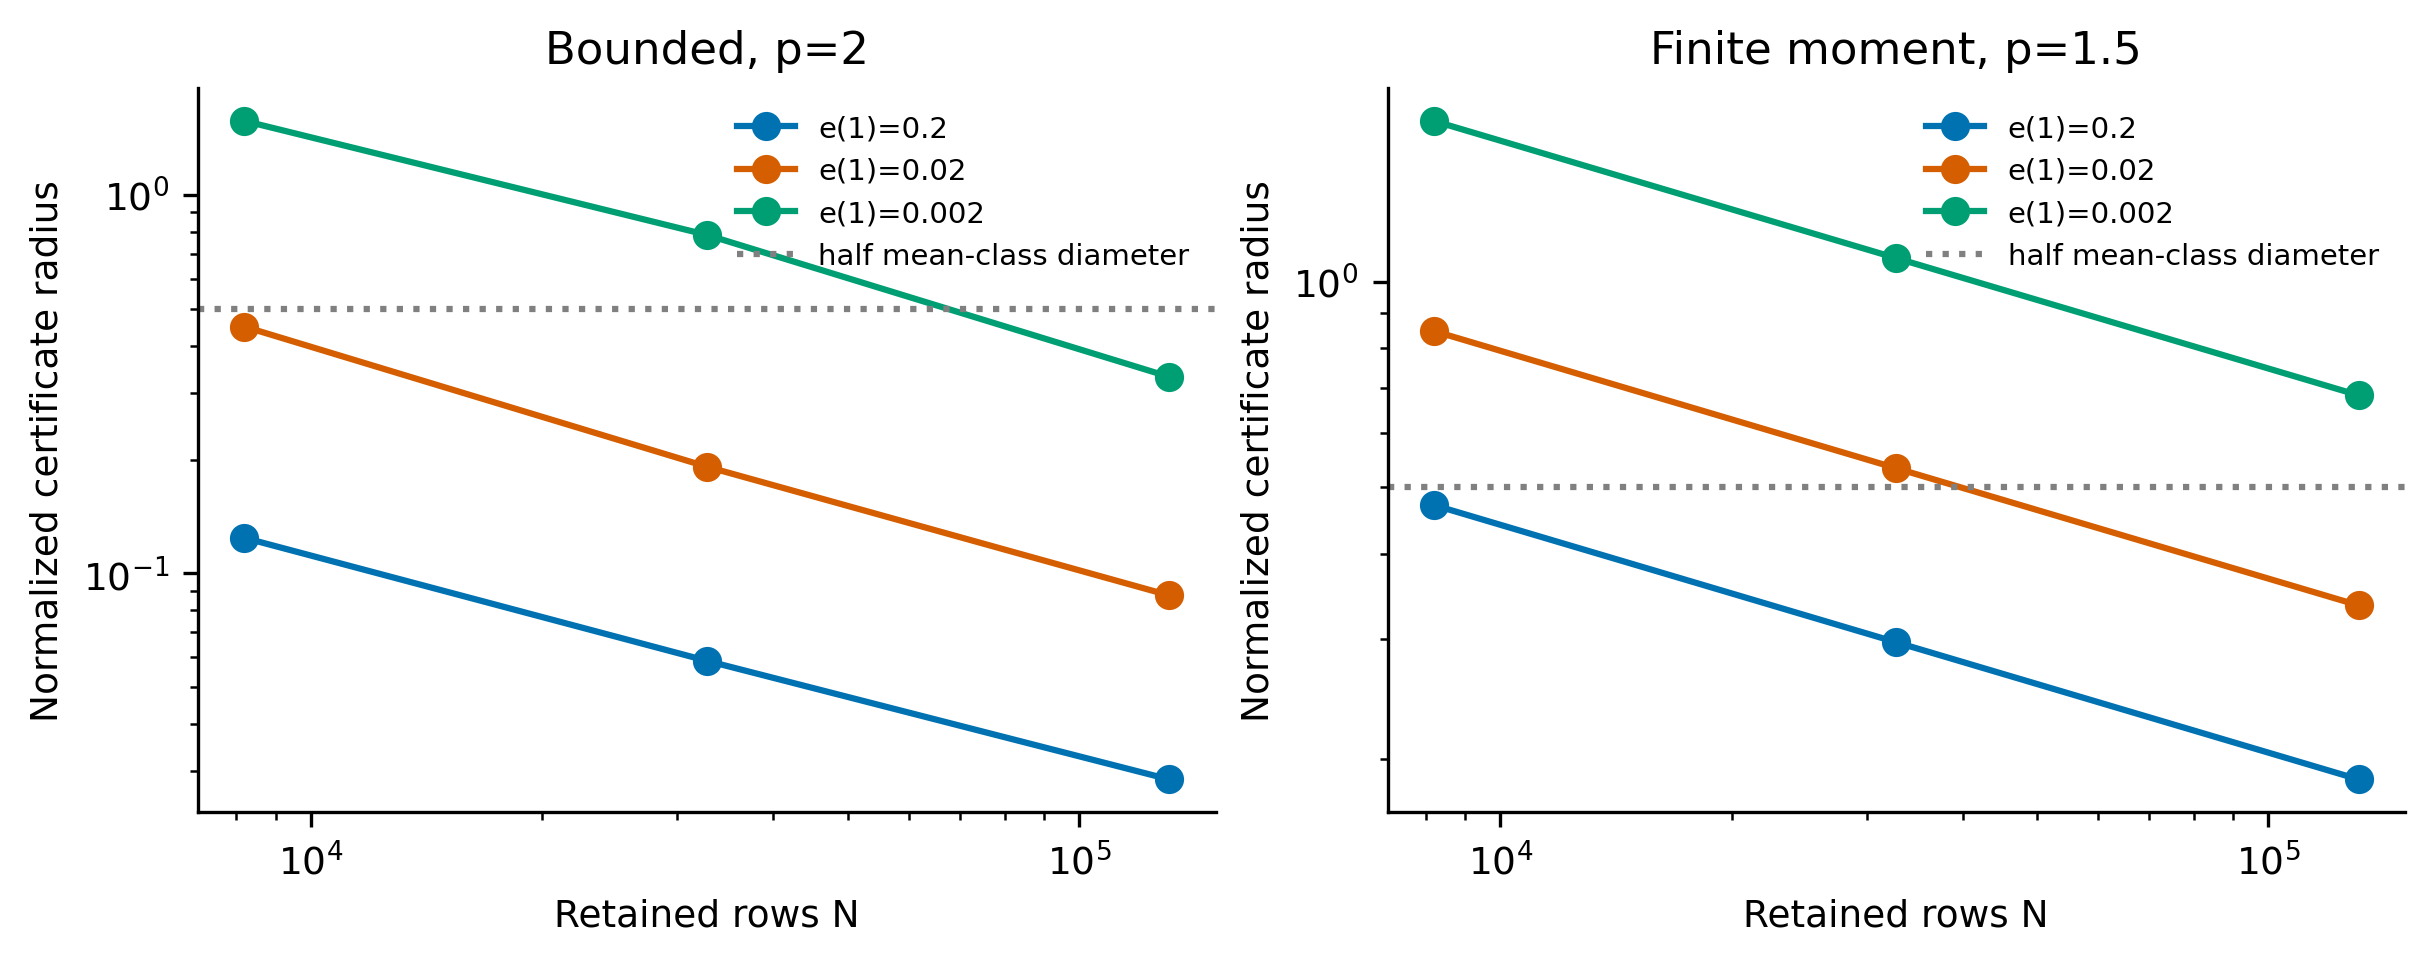
\includegraphics[width=\linewidth]{figures/design_v1/analytic_evidence_cost.png}
\caption{Deterministic normalized certificate radii at subgroup mass near .1,
available coloring count 2, family size 16 and total failure budget .05.
The bounded panel permits a design-only choice among truncation, Hoeffding
and Bernstein. The finite-moment panel uses the declared Pareto-source
residual envelope. No Monte Carlo error bars apply.}
\label{fig:post-cost}
\end{figure}

\begin{figure}[ht]
\centering
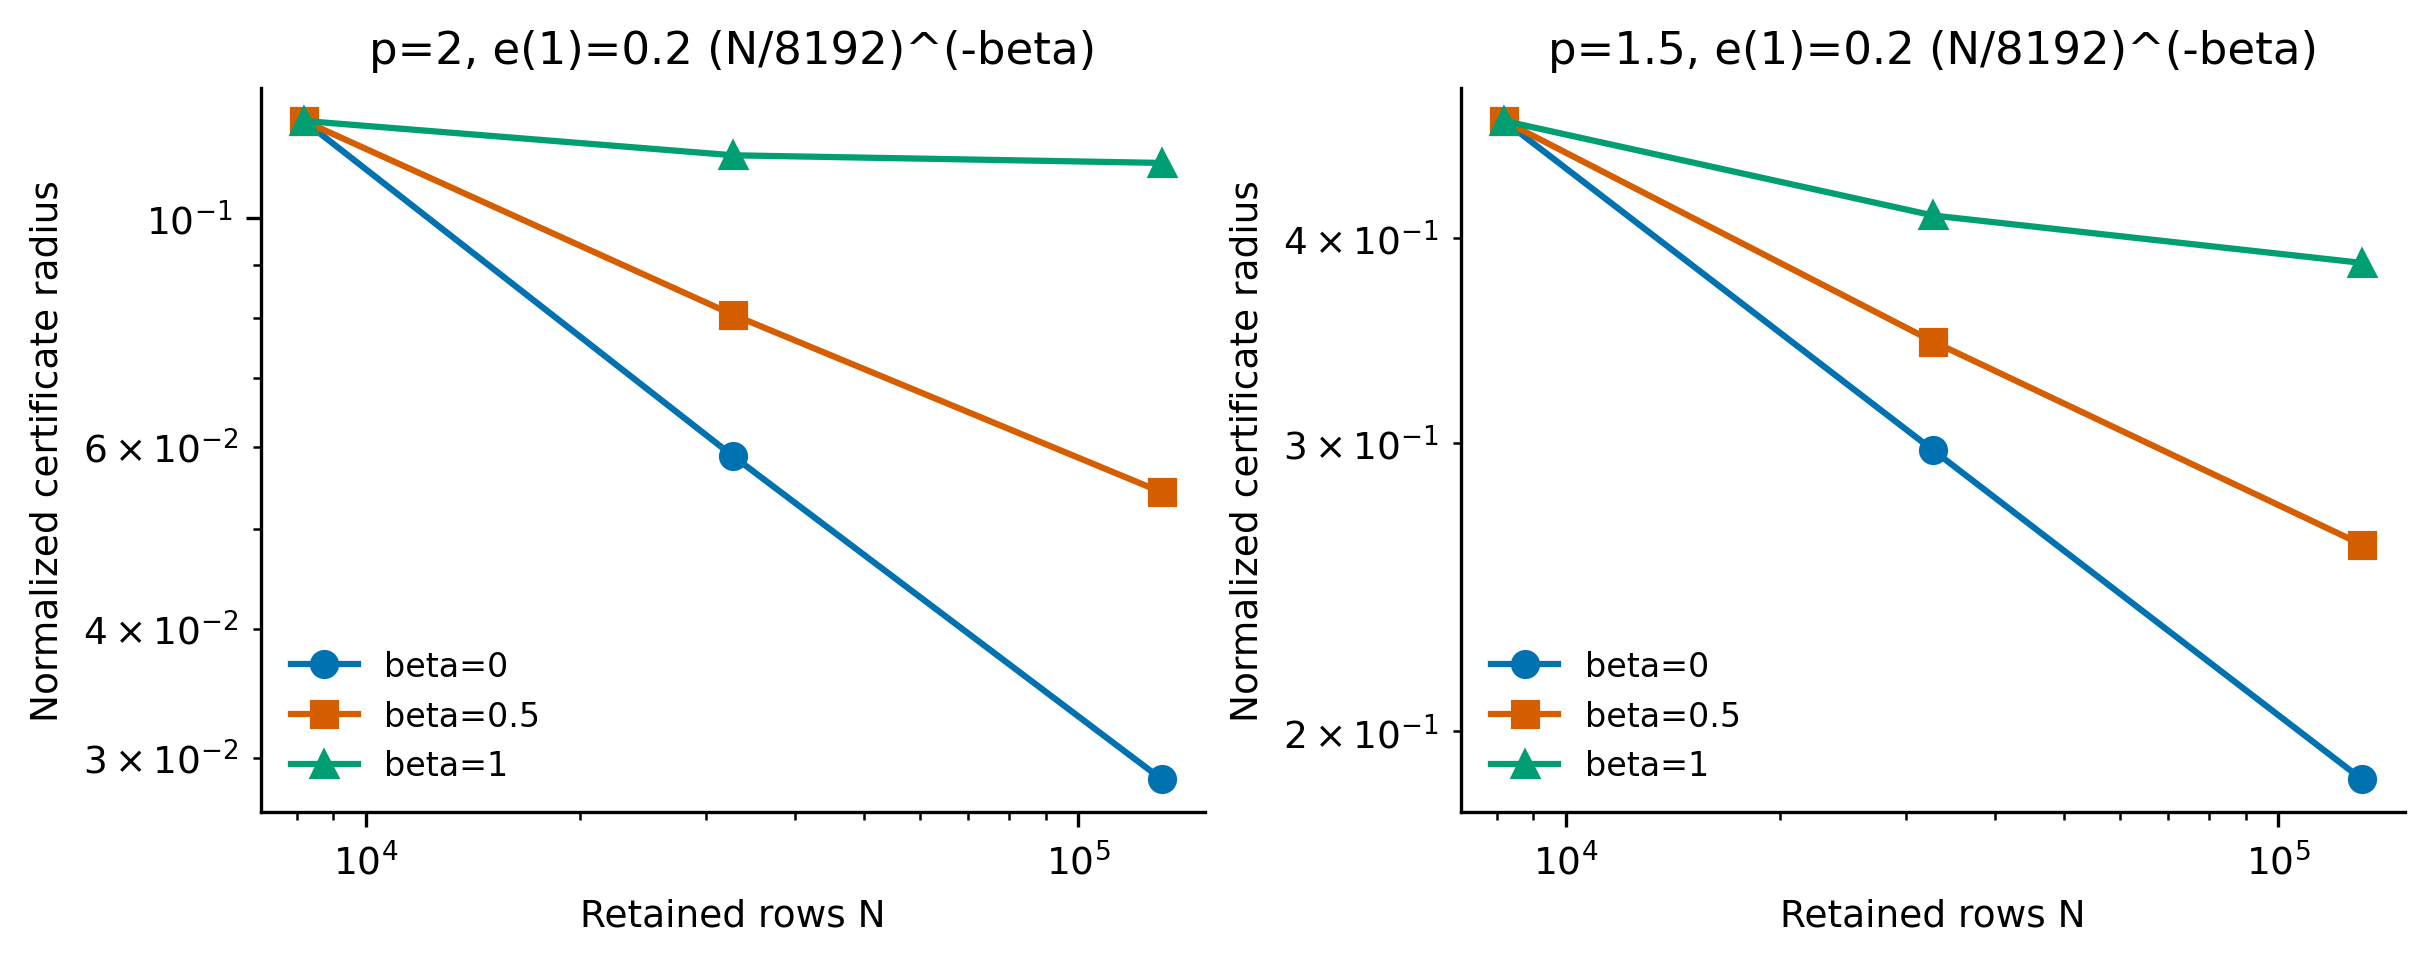
\includegraphics[width=\linewidth]{figures/design_v1/analytic_declining_overlap.png}
\caption{Declining exposure can offset growing row count. The design-only
schedule is $\epsilon_N=.2(N/8192)^{-\beta}$, with the other quantities as in
Figure~\ref{fig:post-cost}. These are procedure-specific sufficient radii,
not a sharp necessary cost or an empirical result for arbitrary weak overlap.}
\label{fig:post-declining}
\end{figure}

\subsection{Contrasts, power boundaries and the complete pipeline}

E3 compares 16 direct signed contrasts with differences of 20 distinct joint
level coordinates, including the four shared baselines only once. Both
constructions spend the same total $\delta$. Changed-support fractions are
.02,.1 and 1, crossed with the two overlap and outcome regimes. Deterministic
controls at step sizes .1,.25,.5 and 1 confirm that shrinking a signed update
scales signal and radius together. This control is not four new data sets.

All 108 primary E3 diagnostics cover 300/300 complete families, with no observed
false claim. In the full-support, moderate-overlap bounded cell, a direct
contrast certifies at least one true positive improvement in 300/300 logs;
the deduplicated joint-level difference certifies none. Mean per-trial
coordinate widths are .0066724 and .0450457 respectively under the same total
confidence budget. Every other cell has zero positive-improvement detections
for COMET, including the smaller-support cells whose raw intervals are
narrower. Thus cancellation can support a useful comparison, but a smaller
raw contrast interval alone is not evidence of higher sign-certification
power. The matched contrast-aware generic construction recovers the same
result. Noninferiority is a separate endpoint and may be easy for tiny raw
changes simply because their known feasible range is small.

E4 fixes a normalized subgroup of mass near .1, risk threshold .4 and true
gaps $\{-.10,-.03,0,.03,.10,.20\}$ in each of four environments. All 24
cells remain included. Detection, false-safe and false-violation decisions
must be interpreted alongside the known design-only $2r$ sufficient boundary;
the procedure never receives the true gap.

E5 learns nuisance functions on 4,096 training rows and discovers at most four
rules of depth at most four and minimum design mass .02 on 8,192 independent
discovery rows. At most eight policies are frozen before 32,768 certification
rows. The risk threshold is .32, utility noninferiority margin .01, service
floor .2 and capacity ceiling .6. The full deduplicated risk-plus-utility family,
typically 47 coordinates, replaces the 16-query validity family. Comparisons
include point constraints, diagnostic in-sample auditing, independent global
and local certificates, matched generic certificates, fixed slices, abstention
and uncertified status quo. The same independent-pilot candidate library is
used by proper certificate engines. Evaluation of fixed-slice and in-sample
returns uses the primary discovered constraints as well as their own-family
diagnostics.

The required pipeline endpoints are return, return and unsafe, return and
infeasible, and return and safe and useful, together with discovery and
certification of a true violation. Utility, utility gain, service, risk
violation and oracle-feasible/robust-slack comparators are evaluation-only.
Conditional unsafe-given-return is separately descriptive. Abstaining in
every trial and rejecting all service cannot count as useful success.
The incomplete E4--E5 outcomes are withheld from performance conclusions
until their fixed counts and analyses are complete.

The single selected real-covariate extension, E6 on ACS California 2018,
remains data-blocked after official-source DNS failure, HTTP403 and a browser
timeout. No E6 trial or replacement data set is reported. Its target is a
fixed-population selective-label moment, not a causal effect of selection
on income. This external limitation does not alter the synthetic protocols.

\section{What the certificates support}

The theorem constructs simultaneous intervals for heterogeneous signed
moments when exact supported exposure laws, a sufficient conditional graph
and legal residual moments are supplied. Its practical resolution depends
on the particular query. A small active region can avoid irrelevant global
weights and graph connections, as the first-half E2 comparison demonstrates.
A small subgroup also contains less relevant evidence, and a small policy
step scales its signal along with its radius. Neither locality nor clipping
guarantees useful decisions in every supported design.

The completed E1 grid separates these issues empirically. The coverage
diagnostics pass throughout, including every heavy-tail cell with zero
detected violations. Stronger bounded inference recovers detection in
settings where Hoeffding or pure truncation does not. Consequently an
uninformative but valid interval should be interpreted as insufficient
evidence under its envelope and graph budget. It does not establish that
the query is safe, or that every valid method must be equally uninformative.
The scoped lower bound identifies an obstruction through subgroup mass,
exposure and clique replication; its expected-risk conclusion does not turn
our sufficient radii into exact information limits.

The same local information is available to the strongest matched comparator.
Its equality with COMET locates the contribution in the signed-moment
formulation, target-specific evidence-cost analysis, scoped limits and
decision contract. The experiments do not support a separate estimator
superiority claim over a fully informed generic graph method. Catoni and
OPE comparisons are restricted to their theorem-compatible submodels;
the differing guarantees and assumptions remain part of the comparison.

Independent discovery permits a random finite audit family to be frozen
before certification. It does not protect all unsearched subgroups.
Similarly, finite-policy certification controls return and unsafe under
the specified risk family. It does not promise frequent return, improved
utility, conditional risk at the same $\delta$, or future deployment safety.
The complete-pipeline results must therefore report baseline returns,
nonbaseline utility and service alongside the joint safe-and-useful event.
The E4 gap study further separates primary-query power from family-any
discovery. Its tested heavy-tail and weak-overlap environments provide no
primary-query certification. E5 remains in progress in this revision; its
partial outcomes do not enter the conclusions here.

The source graph and moment envelope are substantive model inputs.
Their declarations cannot rule out a hidden common shock or certify an
unknown tail scale from one evaluation log. The numerical implementation
also remains distinct from a formally verified outward-rounded realization
of the real-arithmetic proof. These boundaries define the experiments'
scope. The blocked ACS extension leaves real-covariate validation absent;
it does not supply evidence against or in favor of a causal social
intervention.

\section{Conclusion}

Counterfactual moment certification depends on the signed query, supported
residual moments and a sufficient graph of the randomness entering its
score. Explicit clipping bias and graph concentration yield a certificate
without equal row means or repeated independent macro-blocks. Query-local
analysis identifies the relevant costs, and direct contrasts preserve the
cancellation in a policy comparison. The empirical validity grid shows both
useful bounded inference and severe limits in the tested heavy-tail regimes.
Decision evidence must meet a further standard: the full risk and utility
family must support safe, useful return under fair strong comparisons.


\paragraph{Reproducibility.}
The new implementation and source graph are separate modules, isolated from
the frozen historical science. The complete historical C-STAT
delivery remains anchored at \texttt{ca5bb878}; its configuration, 6,000
checkpoints and seventeen primary comparisons are unchanged. Separate committed
protocols bind the new study configurations, seeds, applicability and numerical
rules. Completed checkpoints are immutable and incomplete identifiers alone
are resumed. The completed program contains 28,600 primary units and 1,700
supplementary units; the reserved 1,000-unit E6 extension is data-blocked.
Read-only diagnostics independently reconstruct all E1--E4 interval records
and E5 selection endpoints without regenerating outcomes. The analytic maps use the 49-point production grid and generate
no outcomes. The independent Overleaf repository is not modified.

\paragraph{Use and interpretation.}
An exposure law, source graph or moment envelope is a substantive assumption,
not a property conferred by passing input validation. A finite-population
selective-label benchmark would not establish a causal effect of selection on
income. No statement here guarantees future-distribution or long-term safety.

\paragraph{AI assistance.}
AI tools assisted derivation, implementation, source review and drafting.
The recorded proofs and checks are reviewable evidence, not a claim of formal
machine verification or independent author sign-off.

\begin{thebibliography}{9}
\bibitem{angelopoulos2025ltt}
A. N. Angelopoulos, S. Bates, E. J. Cand\`es, M. I. Jordan, and L. Lei.
Learn then test: Calibrating predictive algorithms to achieve risk control.
\emph{The Annals of Applied Statistics}, 19(2):1641--1662, 2025.
\href{https://doi.org/10.1214/24-AOAS1998}{doi:10.1214/24-AOAS1998}.
\bibitem{thomas2015hcpi}
P. Thomas, G. Theocharous, and M. Ghavamzadeh.
High Confidence Policy Improvement.
In \emph{Proceedings of ICML}, PMLR 37:2380--2388, 2015.
\href{https://proceedings.mlr.press/v37/thomas15.html}{Publisher record}.
\bibitem{janson2004}
S. Janson. Large deviations for sums of partly dependent random variables.
\emph{Random Structures \& Algorithms}, 24(3):234--248, 2004.
\href{https://doi.org/10.1002/rsa.20008}{doi:10.1002/rsa.20008}.
\bibitem{bhatt2022}
S. Bhatt, G. Fang, P. Li, and G. Samorodnitsky.
Nearly Optimal Catoni's M-estimator for Infinite Variance.
\emph{Proceedings of ICML}, PMLR 162:1925--1944, 2022.
\href{https://proceedings.mlr.press/v162/bhatt22b.html}{PMLR source}.
\bibitem{ope2021}
N. Karampatziakis, P. Mineiro, and A. Ramdas.
Off-Policy Confidence Sequences.
\emph{Proceedings of ICML}, PMLR 139:5301--5310, 2021.
\href{https://proceedings.mlr.press/v139/karampatziakis21a.html}{PMLR source}.
\bibitem{ope2024}
I. Waudby-Smith, L. Wu, A. Ramdas, N. Karampatziakis, and P. Mineiro.
Anytime-valid off-policy inference for contextual bandits.
arXiv:2210.10768v3, 2024 (first posted 2022).
\href{https://arxiv.org/abs/2210.10768v3}{Versioned preprint}.
\bibitem{esguard2026}
M. Kim, H. Byun, and B. Jang.
Bias-Aware Guardrail Selection Under Network Interference.
arXiv:2610.36702v1, 2026.
\href{https://arxiv.org/html/2610.36702v1}{Versioned source}.
\end{thebibliography}
\appendix
\section{Proofs for the heterogeneous conditional-graph model}
\label{app:post-proofs}

Throughout this appendix probabilities and expectations condition on the
legitimate field $\mathcal D$ of Section~\ref{sec:post-cstat-theory}. All
quantities selected from an independent training/discovery pool are fixed in
this conditional probability space. We suppress the coordinate subscript
$\theta$ where doing so introduces no ambiguity.

\subsection{Identification and legal raw residual moments}

Finite enumeration over the supported exposure law gives
\begin{align}
 \mathbb E R_u
 &=\sum_{s:e_{us}>0}e_{us}\frac{d_{us}}{e_{us}}
       \mathbb E[Y_u-\widehat\mu_{us}\mid S_u=s,\mathcal D]
   =\sum_s d_{us}(\mu_{us}-\widehat\mu_{us}),
 \label{eq:post-proof-dr}\\
 M&=D+B^{-1}\sum_u\mathbb E R_u.
 \nonumber
\end{align}
A zero coefficient contributes zero without forming $0/0$. A nonzero
coefficient at zero exposure is unsupported. The conditional mean identity
used in~\eqref{eq:post-proof-dr} must describe the desired counterfactual
mean; a probability array by itself does not establish that identification.
The nuisance need not equal these means, and the row distributions need not
coincide.

Similarly,
\begin{equation}
 \mathbb E|R_u|^p
 =\sum_{s:e_{us}>0}|d_{us}|^p e_{us}^{1-p}
       \mathbb E[|Y_u-\widehat\mu_{us}|^p\mid S_u=s,\mathcal D]
 \leq v_u.
 \label{eq:post-proof-raw-moment}
\end{equation}
The absolute value includes the sign of a contrast. For bounded responses,
$|Y_u-\widehat\mu_{us}|\leq\max\{|L_{us}-\widehat\mu_{us}|,
|U_{us}-\widehat\mu_{us}|\}$. A midpoint fit on $[0,1]$ gives the bound
$1/2$, which every eligible method retains. For a location plus noise,
Minkowski gives
\begin{equation}
 \|Y_u-\widehat\mu_{us}\|_p
 \leq|\mu_{us}-\widehat\mu_{us}|+\|\xi_{us}\|_p.
 \label{eq:post-proof-location}
\end{equation}
A known location class and known noise norm therefore supply a legal raw
residual envelope. For a sum of primitive noises, its norm is at most the sum
of their coefficient-weighted norms. No empirical tail-scale estimate is
silently promoted to a known bound.

\subsection{Sharp clipping bias and truncated fluctuations}

\begin{lemma}[Sharp clipping-bias inequality]
\label{lem:post-bias}
For $p>1$, $\tau>0$ and every $x\in\mathbb R$,
\begin{equation}
 |x-T_\tau(x)|\leq
 \frac{(p-1)^{p-1}}{p^p}\tau^{1-p}|x|^p.
 \label{eq:post-proof-bias}
\end{equation}
The constant is sharp.
\end{lemma}
\begin{proof}
For $|x|\leq\tau$ the left side is zero. Otherwise put $z=|x|/\tau>1$.
The ratio in question is $(z-1)/z^p$, whose derivative has the sign of
$p-(p-1)z$. Its maximum is attained at $z=p/(p-1)$ and equals
$(p-1)^{p-1}/p^p$. An atom at that value achieves equality. Taking expectations
in~\eqref{eq:post-proof-bias} gives
$|\mathbb E T_\tau(R)-\mathbb E R|\leq c_pv\tau^{1-p}$.
\end{proof}

For $1<p\leq 2$, checking separately $|x|\leq\tau$ and $|x|>\tau$ gives
\begin{equation}
 T_\tau(x)^2\leq\tau^{2-p}|x|^p,
 \qquad
 \operatorname{Var}(T_\tau(R))\leq v\tau^{2-p}.
 \label{eq:post-proof-second}
\end{equation}
Moreover
$|T_\tau(R)-\mathbb E T_\tau(R)|\leq 2\tau$.
The centering is used only in the proof, not in the estimator. The second
moment inequality cannot be reused for $p>2$: $x=.1$, $\tau=1$ and $p=3$
give $.01>.001$. A centered-noise bound is also insufficient for clipping
bias: a deterministic raw residual $R=2\tau$ has zero centered moment but
clipping bias $\tau$.

\subsection{Source graphs, support restriction and the MGF}

Suppose the declared primitives are jointly independent conditional on
$\mathcal D$, and every whole row vector is measurable in its listed
primitives and $\mathcal D$. Connect every pair of rows whose primitive lists
intersect. Disjoint vertex sets with no crossing edge use disjoint primitive
collections; their generated sigma-fields are independent. This proves the
strong conditional dependency-graph property. Shared outcome noise, logging
randomness and retained response channels all enter this construction.
Pairwise covariance alone does not establish the property.

For any design-active subset, disjoint vertex sets with no induced crossing
edge also have no crossing edge in the original graph. Their independence is
therefore retained. Removing an inactive vertex never removes a primitive
shared by two retained vertices. A proper color class has no internal edges,
so its row variables are jointly independent. For more than two vertices,
this follows by separating one vertex from the remainder and applying the
graph property inductively.

For a centered random variable $X$ with $|X|\leq b$ and
$\mathbb E X^2\leq a$, expansion of the exponential gives, when
$b|\lambda|<3$,
\begin{align}
 \mathbb E e^{\lambda X}
 &\leq 1+\frac{\lambda^2a}{2}
          \sum_{j=0}^\infty\left(\frac{b|\lambda|}{3}\right)^j,
 &\log\mathbb E e^{\lambda X}
 &\leq\frac{\lambda^2a}{2(1-b|\lambda|/3)}.
 \label{eq:post-proof-bernstein-mgf}
\end{align}
Here $|\mathbb E X^k|\leq ab^{k-2}$ and
$k!\geq 2\cdot 3^{k-2}$ for $k\geq 2$ justify the series bound.

Let $X_u=T_{\tau_u}(R_u)-\mathbb E T_{\tau_u}(R_u)$,
$A=\sum_uv_u\tau_u^{2-p}$ and $\tau_{\max}=\max_u\tau_u$.
For a verified proper $\chi$-coloring $C_1,\ldots,C_\chi$, H\"older's
inequality followed by within-color independence yields
\begin{align}
 \mathbb E e^{\lambda\sum_uX_u}
 &\leq\prod_{j=1}^\chi
    \left(\mathbb E e^{\chi\lambda\sum_{u\in C_j}X_u}\right)^{1/\chi},
 \nonumber\\
 \log\mathbb E e^{\lambda\sum_uX_u}
 &\leq\frac{\chi\lambda^2A}
              {2(1-(2/3)\chi\tau_{\max}|\lambda|)}.
 \label{eq:post-proof-graph-mgf}
\end{align}
Different color sizes and different row means do not alter this argument.
There is no decomposition into independent macro-block observations.

Write $V=\chi A$ and $c=(2/3)\chi\tau_{\max}$. The sub-gamma bound
$\log\mathbb E e^{\lambda\sum X_u}\leq
V\lambda^2/(2(1-c|\lambda|))$ implies
\begin{equation}
 \Pr\left(\left|\sum_uX_u\right|>
                \sqrt{2Vt}+ct\right)\leq 2e^{-t}.
 \label{eq:post-proof-tail}
\end{equation}
For $V>0$, substitute
$\lambda=\sqrt{2t/V}/(1+c\sqrt{2t/V})$ into Chernoff's inequality, and
apply the same calculation to $-\sum X_u$. The deterministic case is direct.
Combining~\eqref{eq:post-proof-tail} with the summed absolute bias from
Lemma~\ref{lem:post-bias}, and dividing by the original normalizer $B$, proves
the coordinate claim in Theorem~\ref{thm:post-core}. A finite union bound over
$\theta$ proves its family statement. No independence between coordinates,
methods or confidence levels is used.

\subsection{Tuning, locality, contrasts and equivalence}

Conditional on $\mathcal D$, every eligible design-only threshold or engine
choice is fixed, so the proof applies to that choice directly. It does not
require a union bound over candidates in a threshold grid. This reasoning
would not justify selecting by observed errors, observed intersected widths
or evaluation-trained fits. For example, independent Rademacher $X_1,X_2$
become equal conditional on evaluation-derived $\mathcal D=X_1X_2=1$;
conditioning is not an independence repair.

A zero coefficient produces an identically zero residual; dropping it leaves
the known direct term and denominator unchanged. In contrast, replacing $B$
by an active-row count generally changes the estimand. Restricting to the
induced graph proves the locality claim. With $d$ replaced by $\eta d$,
$v$ becomes $\eta^pv$ and $\tau$ becomes $\eta\tau$. The bias, square-root
and range terms each become $\eta$ times their previous value. This proves
Corollary~\ref{cor:post-locality}. A separate-level subtraction comparison
must allocate its total confidence budget to both level families; a paired
contrast uses its signed coefficient directly.

Any generic truncated graph mean with the same deterministic direct term,
residuals, envelopes, support, coloring, thresholds and confidence allocation
has exactly the estimator and radius in~\eqref{eq:post-estimator} and
\eqref{eq:post-radius}. Thus a matched implementation is algebraically equal,
including any common design-only bounded-branch dispatch. Coarser global graph
or global maximum-envelope versions are component ablations rather than
competitors denied available local information.

\subsection{Bounded Hoeffding, Bernstein and colorwise comparisons}

For each supported exposure, the residual lies between the endpoints of
\begin{equation}
 \frac{d_{us}}{e_{us}}[L_{us}-\widehat\mu_{us},
                       U_{us}-\widehat\mu_{us}],
 \label{eq:post-proof-actual-range}
\end{equation}
with endpoint order reversed when $d_{us}<0$. Taking the extrema over all
supported exposures gives $[\ell_u,u_u]$ and width $w_u=u_u-\ell_u$.
Zero-coefficient supported exposures contribute the value zero. Observed
sample extrema are not substituted for these known ranges.

For a variable $Z$ supported on $[a,b]$, write
$f(\lambda)=\log\mathbb E\exp(\lambda(Z-\mathbb EZ))$. Under exponential
tilting, $f''(\lambda)$ is the variance of a distribution still supported on
$[a,b]$. For any such distribution, variance is at most
$\mathbb E[(Z-(a+b)/2)^2]\leq(b-a)^2/4$. Integrating twice from
$f(0)=f'(0)=0$ proves Hoeffding's MGF bound
$f(\lambda)\leq\lambda^2(b-a)^2/8$ for either sign of $\lambda$.
Applying this rowwise and using the same coloring/H\"older step
bounds the summed log MGF by $\chi\lambda^2\sum_uw_u^2/8$.
A two-tail Chernoff argument gives~\eqref{eq:post-hoeffding}.
The raw second moment is bounded by
\begin{equation}
 v_u^{(2)}=\sum_{s:e_{us}>0}\frac{d_{us}^2}{e_{us}}
            \max\{|L_{us}-\widehat\mu_{us}|,
                   |U_{us}-\widehat\mu_{us}|\}^2.
\end{equation}
Variance is also at most $w_u^2/4$, so its minimum with $v_u^{(2)}$ is valid.
The centered residual has absolute magnitude at most $w_u$. Substitution into
\eqref{eq:post-proof-bernstein-mgf}--\eqref{eq:post-proof-tail}, with scale
$c=\chi\max_uw_u/3$, proves~\eqref{eq:post-bernstein}.
Both bounded radii use the same actual nuisance-dependent support and
confidence budget as the main method.

For completeness, a colorwise independent truncation comparator is valid
with positive budgets $\delta_j$ satisfying $\sum_j\delta_j\leq\delta_\theta$.
For color $C_j$, let $A_j=\sum_{u\in C_j}v_u\tau_u^{2-p}$,
$t_j=\log(2/\delta_j)$ and $\tau_{\max,j}=\max_{u\in C_j}\tau_u$.
By an independent Bernstein argument and a union bound its total radius is
\begin{equation}
 \frac 1B\sum_j\left[
     c_p\sum_{u\in C_j}v_u\tau_u^{1-p}
     +\sqrt{2A_jt_j}+\frac 23\tau_{\max,j}t_j\right].
 \label{eq:post-proof-colorwise}
\end{equation}
Every color is retained. Equivalently, color-average estimators are recombined
with their actual color-size weights divided by $B$. Equal averaging of
unequal colors or omission of a difficult color changes the target.

In the deterministic A fixture~\eqref{eq:post-A-fixture}, every residual range
has width one and the graph is empty. Direct substitution in
\eqref{eq:post-hoeffding} gives its stated radius. On
$|\widehat M-M|\leq r_H$, the lower endpoint is at least
$M-2r_H>.2$, proving the analytic detection implication without drawing data.

\subsection{Observation thinning and a scoped lower bound}
\label{app:post-lower}

We give the explicit experiment behind Proposition~\ref{prop:post-lower}.
The subgroup has $g=N\pi$ rows arranged into $n=g/\chi$ cliques. In clique $j$,
draw independent $A_j\sim\operatorname{Bernoulli}(\epsilon)$ and
$V_j\sim\operatorname{Bernoulli}(t)$, independently between cliques. Copy them
within the $\chi$ rows. Let
\begin{equation}
 t=\min\{1,(2n\epsilon)^{-1}\},\qquad
 a=\min\{H/t,\nu t^{-1/p}\},\qquad
 \eta=at=\min\{H,\nu t^{(p-1)/p}\}.
 \label{eq:post-proof-thinning}
\end{equation}
Under sign $\sigma\in\{-1,+1\}$ define
$Y_j(0)=b$ and $Y_j(1)=b+\sigma aV_j$. Logging is independent of potential
responses. Observe the exposure and the selected response. The full logging
law consists of independent Bernoulli clique assignments, and the target joint
policy assigns action one throughout the subgroup. Outside-subgroup data have
the same distribution under both signs and carry no sign information.

Known nuisance $b$ has
$\mathbb E|Y_j(1)-b|^p=a^pt\leq\nu^p$. The normalized subgroup target is
$\theta_\sigma=b+\sigma\eta$, and its raw IPW residual moment is at most
$\epsilon^{1-p}\nu^p$. To keep conditional means in $[0,1]$, choose $b=1/2$
and $H\leq 1/2$. The response amplitudes need not be bounded: bounded conditional
means and finite moments are distinct assumptions. This construction is not a
bounded-response lower bound.

Let $P_+$ and $P_-$ denote the observable laws. They agree unless at least one
clique has $A_j=V_j=1$. On that event positive and negative spike values are
disjoint. Thus
\begin{equation}
 \operatorname{TV}(P_+,P_-)
   =1-(1-\epsilon t)^n
   \leq n\epsilon t\leq\frac 12.
 \label{eq:post-proof-tv}
\end{equation}
For any estimator $T$, integrate the triangle inequality over the common
part of the two probability measures. Since the parameter distance is
$2\eta$,
\begin{equation}
 \mathbb E_+|T-\theta_+|+\mathbb E_-|T-\theta_-|
 \geq 2\eta(1-\operatorname{TV}(P_+,P_-)).
\end{equation}
The maximum risk is at least half this sum, hence at least
$\eta(1-\operatorname{TV})\geq\eta/2$, proving
\eqref{eq:post-lower}. Multiplying targets by $\pi$ multiplies the risk bound
by $\pi$.

When $2n\epsilon\geq 1$ and the mean cap does not bind, the normalized
lower-bound scale is
\[
2^{-1-(p-1)/p}\,\nu\left(\frac{\chi}{N\pi\epsilon}\right)^{(p-1)/p}.
\]
For the raw
moment it is the same constant times
$\nu\pi^{1/p}(\chi/(N\epsilon))^{(p-1)/p}$.
Equation~\eqref{eq:post-proof-thinning} records mean saturation and small
effective-sample regimes. The integer requirements $N\pi\in\mathbb N$ and
$\chi\mid N\pi$ and the explicit observable experiment are part of the claim.
The sample-size-dependent spike distribution is a minimax construction, not a
prediction for a fixed Pareto simulation.

At exactly zero exposure support, take $A_j=0$ always and
$Y_j(1)=b\pm\min\{H,\nu\}$. The observable laws are identical while the
subgroup targets differ. The same common-measure argument gives maximum
absolute risk at least $\min\{H,\nu\}$. This is nonidentification outside
the supported core model; an IPW certificate is unavailable, and the API
refuses a nonzero target coefficient at zero exposure rather than flooring it.

There is also a simple confidence-width consequence. If a random interval $I$
has coverage at least $1-\alpha$ under each sign, change of measure gives
\begin{equation}
 P_+(\theta_+\in I,\theta_-\in I)
 \geq 1-2\alpha-\operatorname{TV}(P_+,P_-)
 \geq\frac 12-2\alpha.
\end{equation}
Consequently its diameter is at least $2\eta$ with at least the displayed
probability when positive; for a raw target replace $2\eta$ by $2\pi\eta$.
This is a non-sharp two-point consequence. It proves neither optimal
$\log(m/\delta)$ factors nor sharpness for every sparse or connected graph.

\subsection{Decision boundaries and eventwise finite-policy statements}

If a true upper-risk threshold gap is $\gamma=M-a_0>2r$, then on
$|\widehat M-M|\leq r$ the lower endpoint satisfies
$\widehat M-r\geq M-2r>a_0$. The analogous negative-gap condition gives a
safe upper endpoint. Merely assuming $\gamma>r$ is insufficient: the admissible
estimate $\widehat M=M-r$ has lower endpoint $M-2r$.
Analytic sample budgets evaluate the complete radius and this sufficient
boundary. They are not new empirical power observations or necessary
information bounds. Numerical implementations must account for any declared
additional endpoint padding in their actual decision boundary.

For Corollary~\ref{cor:post-selection}, condition first on the independent
discovery pool. Its finite selected family and all subsequent plans are fixed;
the union event of Theorem~\ref{thm:post-core} includes all coordinates used in
audit and selection. On that event every certified risk upper bound is an upper
bound on the true fixed-design risk, and every certified utility lower bound
is a lower bound on its true contrast. Exact service/capacity are deterministic.
Thus a returned policy meeting all these checks is safe and useful in their
declared sense. Any false returned-policy claim is contained in the complement
of the simultaneous event. Integrating the conditional bound proves
$\Pr(\mathrm{return}\ \mathrm{and}\ \mathrm{unsafe})\leq\delta$.
If the return probability is positive, only the general bound
$\Pr(\mathrm{unsafe}\mid\mathrm{return})\leq
\delta/\Pr(\mathrm{return})$ follows. Total abstention cannot count as useful
return; reject-all fails a positive service requirement. No uncertified
fallback is covered by the argument.

The robust-slack and oracle-feasible comparators must be distinguished.
Suppose risk intervals are centered with radii $r^R_{jk}$, and utility contrast
intervals with radii $r^U_j$. On the simultaneous event a candidate $j$ whose
true risks satisfy $R_{jk}\leq b_k-2r^R_{jk}$ has all risk upper bounds feasible.
If its true utility contrast is at least the usefulness threshold plus
$2r^U_j$ and its exact service/capacity are feasible, it enters the certified
library. Selecting a maximal utility lower endpoint then gives
\begin{equation}
 U_{\mathrm{selected}}-U_0
 \geq L^U_{\mathrm{selected}}\geq L^U_j
 \geq U_j-U_0-2r^U_j.
 \label{eq:post-proof-robust-comparator}
\end{equation}
This is the eventwise robust-margin comparator. The oracle best feasible
candidate may have zero constraint slack and fail to enter the certified
library, so~\eqref{eq:post-proof-robust-comparator} is not a universal regret
bound against that different comparator. Neither comparator is supplied to
the certifier or selector as oracle input.

Finally, under simultaneous base-policy intervals, every nonnegative weight
vector summing to one satisfies
$\sum_jw_jL_j\leq\sum_jw_jM_j\leq\sum_jw_jU_j$ on the same event. This is a
deterministic inequality for all weight vectors, including data-selected ones.
A mixture of compatible joint policies is itself a joint policy, and its fixed-
auditor affine moments equal the mixture of the base moments. For signed
affine combinations, reverse the relevant endpoints when multiplying by a
negative coefficient. No new union over mixture weights is needed.
This proves Corollary~\ref{cor:post-mixtures}; it does not identify a fresh
nonlinearly clipped estimate with the mixture of certified base estimates,
or extend to policy-dependent denominators and nonlinear fairness metrics.

\section{Eligibility of the independent strong-baseline anchors}
\label{app:post-iid-anchor}

The homogeneous independent anchor has exact logging law
$e=(3/4,1/4)$, target $q=(1/2,1/2)$, fixed nuisance $1/2$ and weights
$w_s=q_s/e_s\in\{2/3,2\}$. Its response locations are $(.35,.55)$, so its
target is $.45$, threshold $.4$ and gap $.05$. These choices precede any
anchor outcome. Each observed DR score
\[
 X=\frac 12+w_S(Y-\tfrac 12)
\]
has that target; the observed outcome $Y$ alone instead averages under the
logging law. All rows share the same distribution and use independent
sources, so the i.i.d. requirement of the Catoni anchor is substantive.

Catoni requires a centered moment envelope. In the bounded $p=2$ anchor,
$Y\in[0,1]$ gives directly
\[
 \operatorname{Var}(X)\leq
 \mathbb E\!\left[\{w_S(Y-\tfrac 12)\}^2\right]
 \leq\frac 14\sum_s e_sw_s^2.
\]
For the finite-$p$ location-plus-noise anchor, let
$\delta_s=\mu_s-1/2\in[-1/2,1/2]$ and suppose
$\|\xi_s\|_p\leq K$. Here
$K=.1(1.75/(1.75-p))^{1/p}$ and $p=1.5$, with the declared finite-grid
qualification. Since $w_s\geq 1/2$, maximization over the four location
corners yields
\[
 \left|w_s\delta_s-\tfrac 12(\delta_0+\delta_1)\right|
 \leq\tfrac 12\{|w_s-\tfrac 12|+\tfrac 12\}
 =\tfrac 12w_s.
\]
Conditional Minkowski therefore gives
\[
 \mathbb E|X-\mathbb EX|^p
 \leq(\tfrac 12+K)^p\sum_s e_sw_s^p.
\]
This equals the legal raw residual envelope in this particular balanced-target,
midpoint-fit location model. It is not a general inequality replacing a
centered moment by a raw moment. The Catoni implementation also checks its
theorem's sample-size condition and retains its deterministic root-solver
debit.

For bounded OPE, $\mathbb Ew_S=1$ and $w_S\leq 2$ are known from the design,
even if a particular log observes only the smaller weight. The author-code
one-dimensional betting instance receives this design maximum. The 2024
DR/empirical-Bernstein engine receives the same logging law, target and
nuisance, with its own stated predictable-predictor truncation and mixture
parameters. These independent anchors do not authorize applying a row-order
martingale directly to an arbitrary connected source graph.

\section{Prespecified invalid-assumption controls}
\label{app:post-negative-controls}

Four supplementary controls each use 25 complete logs with $N=32768$, one
query and the same two nominal levels. Their configurations precede their
outcomes. Each compares a valid reference under the actual model, an
intentionally invalid interval labeled heuristic, and an honest refusal when
the required premise is not supplied. The invalid output is never promoted
to a certified result. Refusal has no interval and no assessable error rate;
it is not a zero-error observation.

\paragraph{Hidden shared shock.}
Every row has response $.45+H$, where $H\in\{-.25,.25\}$ is a single common
shock. The invalid description supplies an empty graph. The true sufficient
graph is complete, although it need not be stored as a quadratic adjacency
matrix. The valid reference uses a deterministic known target range. A narrow
interval obtained by pretending the rows are independent can be wrong even
though the declared array shapes and probability rows pass validation.

\paragraph{Wrong exposure law.}
The true action-one exposure is $1/5$, generated by an exact five-way lottery;
the invalid input says $1/2$. The target puts probability .8 on action one,
the response locations are $(.2,.8)$ and the nuisance is .5. The true target is
.68. The valid reference receives the true exposure law. A probability array
being normalized does not show that it equals the logger's actual law.

\paragraph{Missing clipping bias.}
The response is $.3+100B$ with $B\sim\operatorname{Bernoulli}(1/200)$,
target equal to logging and nuisance .5. Its mean is .8. At the fixed threshold
$\tau=.01$, the expected clipped DR score is .4901, giving exact clipping
bias .3099. A legal $p=1.5$ raw moment is computed analytically from the two
atoms before sampling. The valid reference pays the complete bias bound even
when it becomes vacuous. The intentionally invalid interval retains the same
estimate but omits this debit. A realized log without an extreme score cannot
justify that omission.

\paragraph{Evaluation-trained nuisance.}
With true exposure $1/5$, target action-one probability .8 and response
locations $(.2,.8)$, the invalid fit sets both state predictions in each row
equal to its observed response. Its weighted residual is zero and its direct
term is the observed outcome, whose mean is .32 rather than the target .68.
The valid reference uses the independent fixed nuisance .5. Conditioning on
the leaked fit does not restore the required identification and independence
conditions. Source provenance can reveal a declared violation, but array
schemas cannot discover every hidden training-data dependency.

Coverage and false claims in these controls describe complete logs under
known intentionally violated premises. They are supplementary diagnostics,
with pointwise Monte Carlo uncertainty, and do not enter the primary validity
families or the historical seventeen-comparison study.

\section{Algebraic evidence-cost maps}
\label{app:post-maps}

The 216 fixed-overlap and 216 declining-overlap configurations evaluate the
full 49-point threshold grid using only design inputs. They retain subgroup
mass, exact exposure, legal residual moments and the available coloring count.
These are procedure-specific sufficient radii and contain no sampled outcomes;
they do not verify a minimax rate or a necessary evidence requirement.

\begin{figure}[ht]
\centering
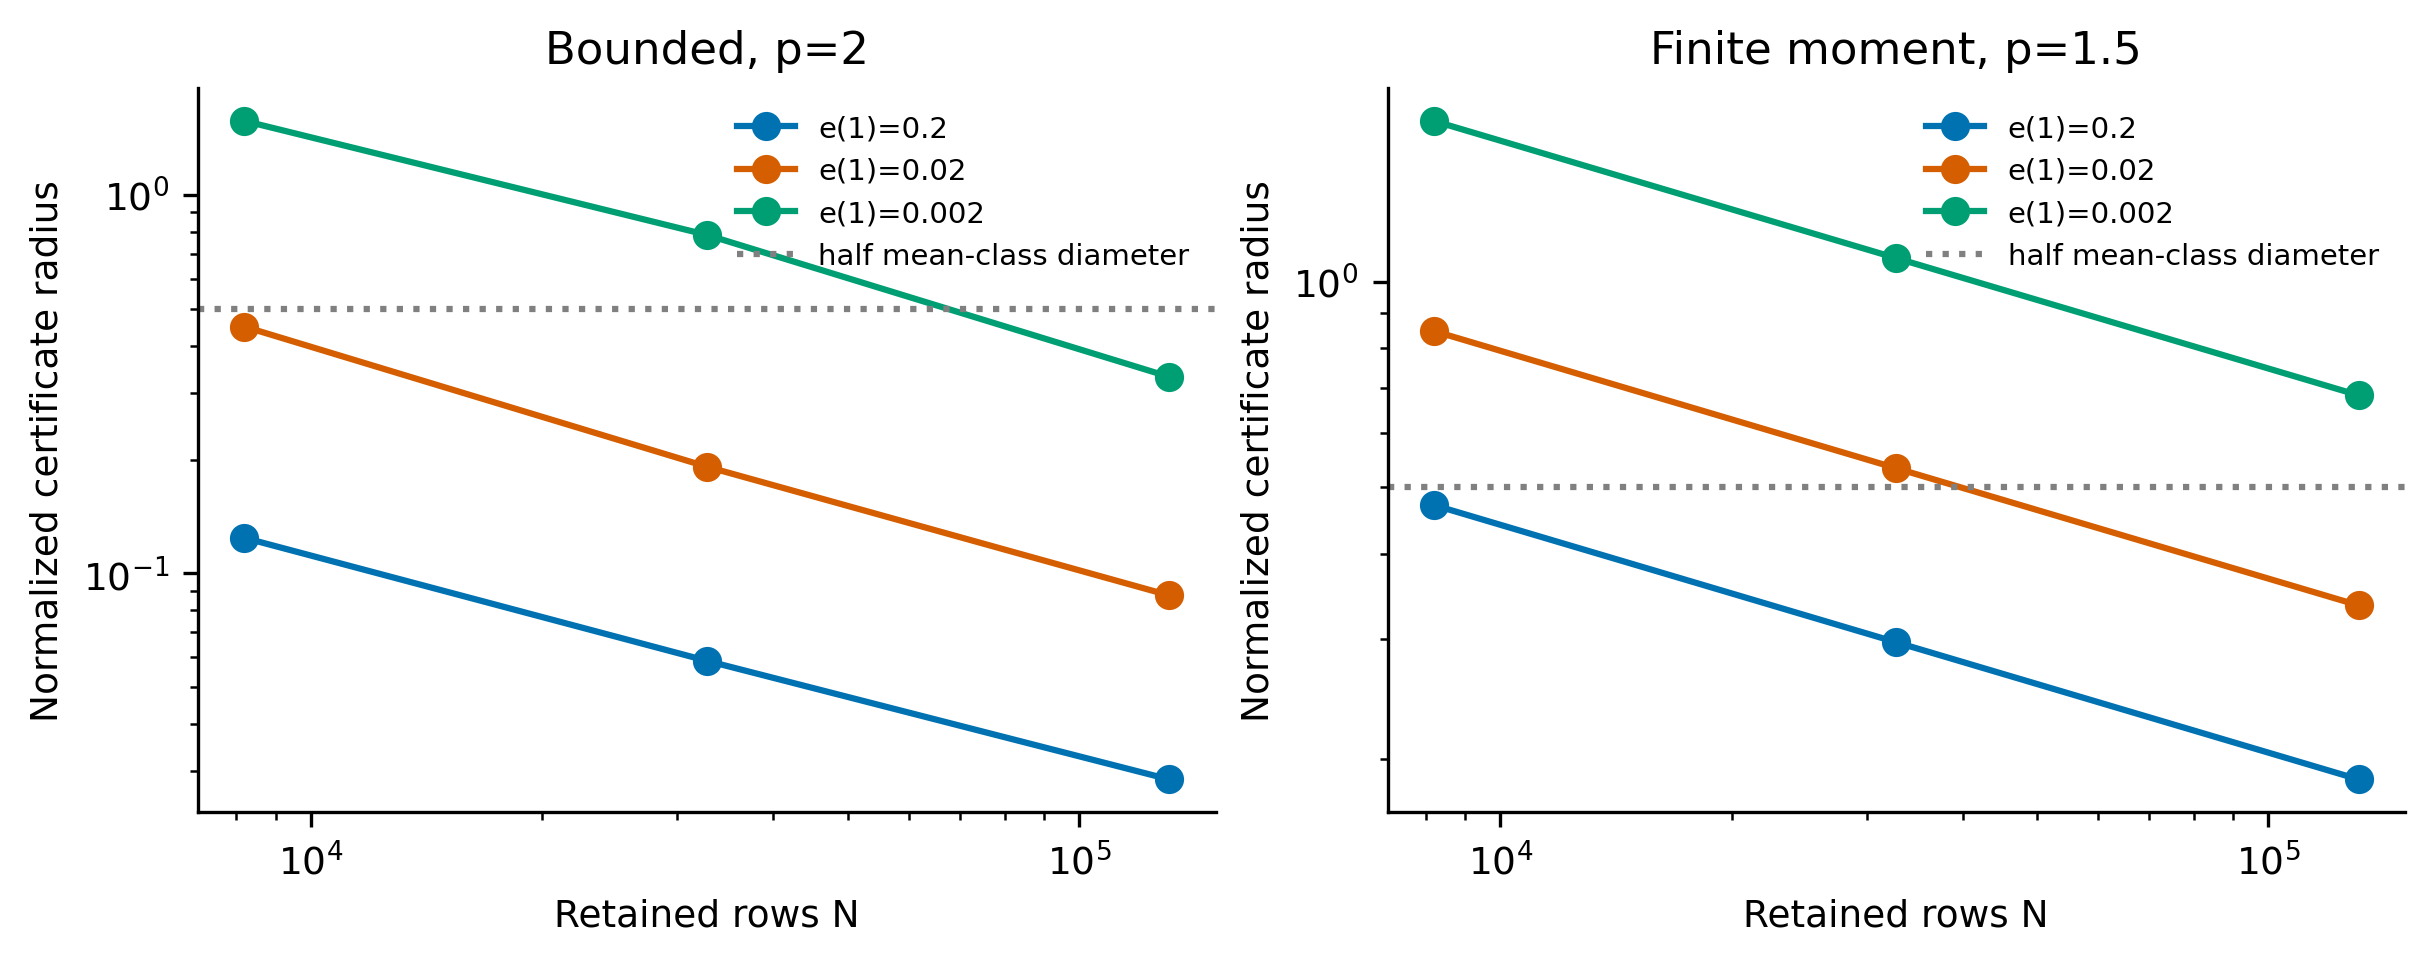
\includegraphics[width=\linewidth]{figures/design_v1/analytic_evidence_cost.png}
\caption{Deterministic normalized certificate radii at subgroup mass near .1,
available coloring count 2, family size 16 and total failure budget .05.
The bounded panel permits a design-only choice among truncation, Hoeffding
and Bernstein. The finite-moment panel uses the declared Pareto-source
residual envelope. No Monte Carlo error bars apply.}
\label{fig:post-cost}
\end{figure}

\begin{figure}[ht]
\centering
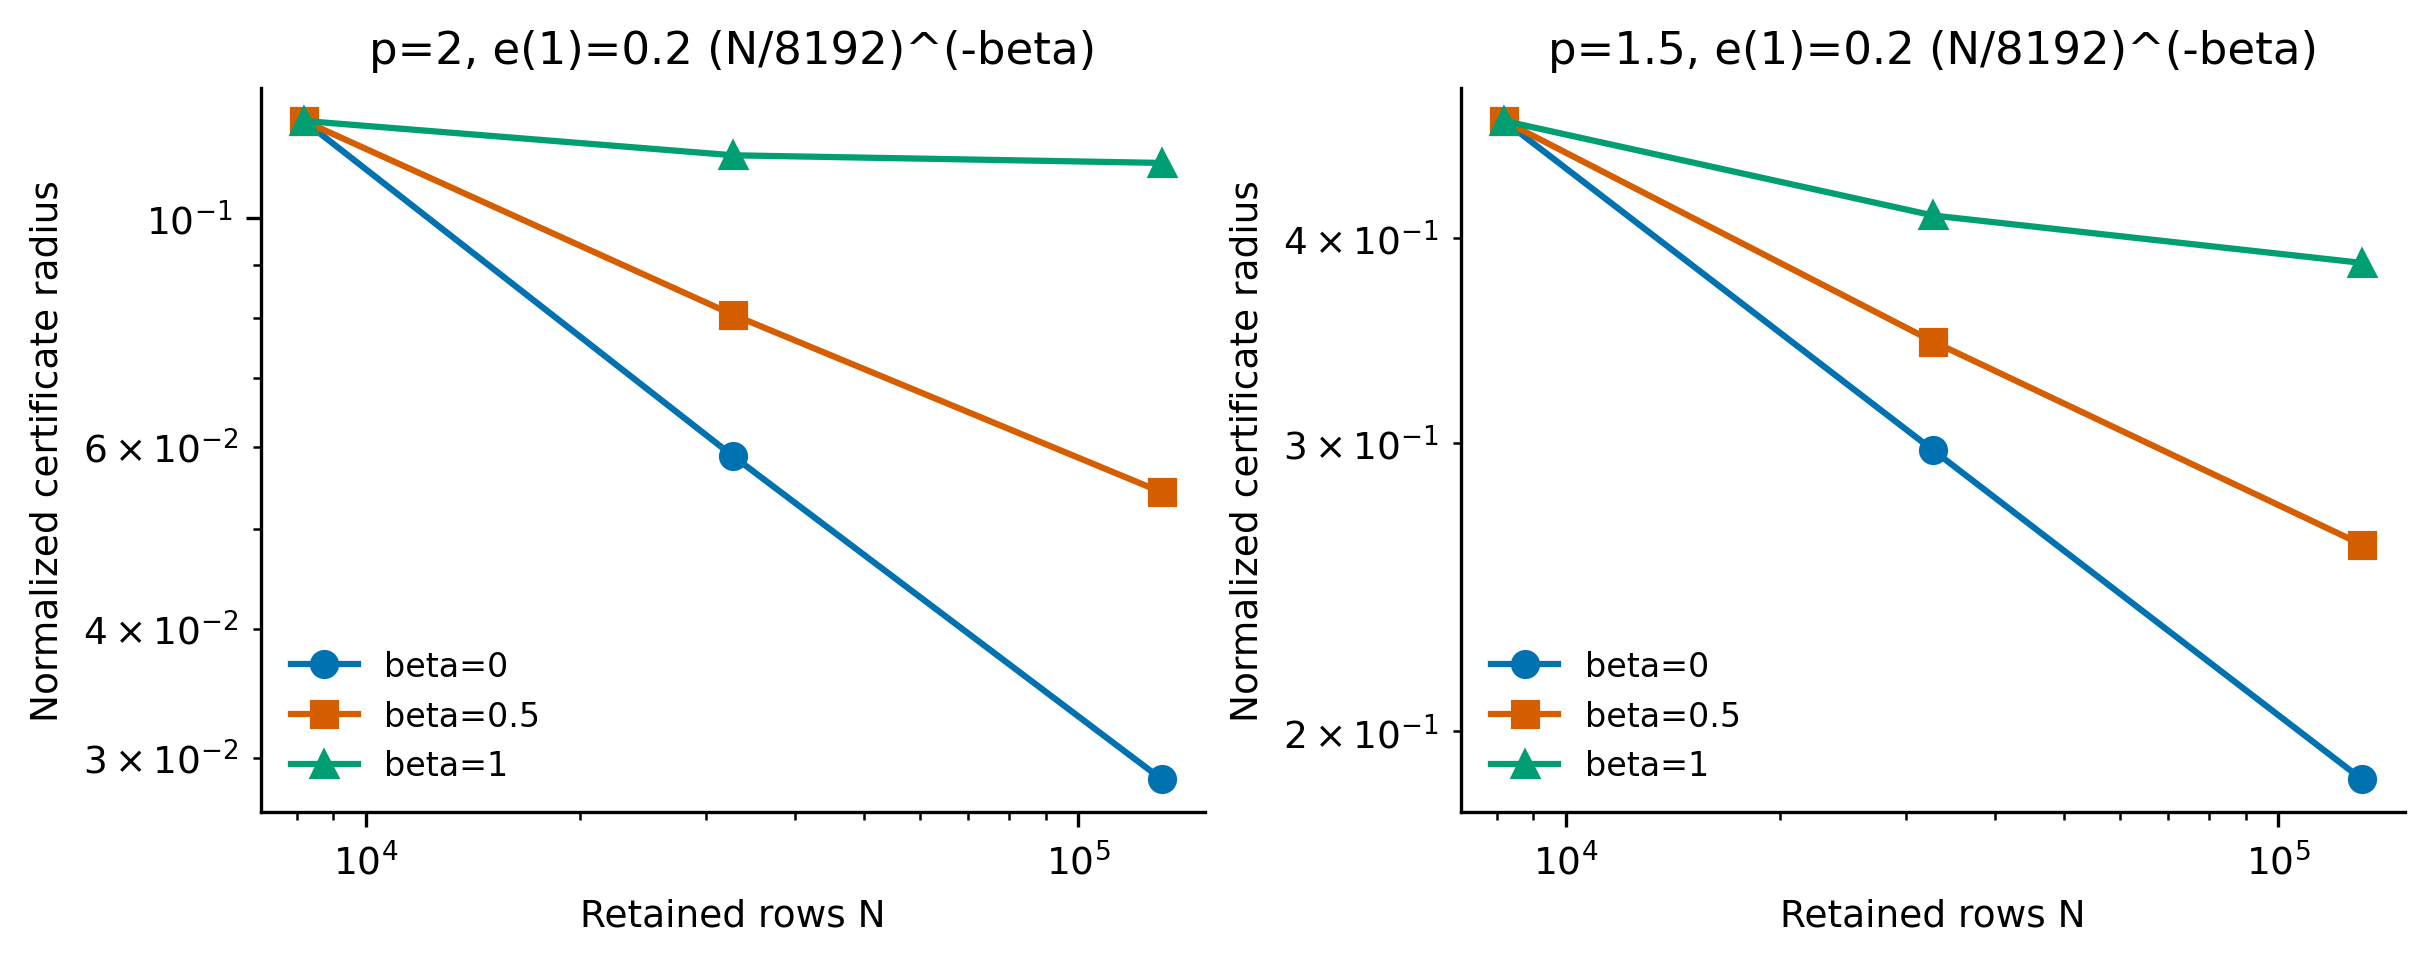
\includegraphics[width=\linewidth]{figures/design_v1/analytic_declining_overlap.png}
\caption{Declining exposure can offset growing row count. The design-only
schedule is $\epsilon_N=.2(N/8192)^{-\beta}$, with the other quantities as in
Figure~\ref{fig:post-cost}. These are procedure-specific sufficient radii,
not a sharp necessary cost or an empirical result for arbitrary weak overlap.}
\label{fig:post-declining}
\end{figure}

\section{Strong-baseline anchors, scaling and assumption controls}
\label{app:post-supplementary}

The supplementary allowance contains 1,600 anchor logs and 100 negative-control
logs, separate from the primary E1--E5 grids. All methods and both confidence
levels share each complete log. The server environment was selected by an
explicit amendment before the first outcome in either supplementary suite;
the unused original local freezes are preserved. No already-started primary
suite changed production environment. All 1,718 returned artifact files were
verified against their server byte hashes; this file count is not a trial count.

\subsection{Theorem-compatible strong comparisons}

The homogeneous IID anchor has $N=32768$, one coordinate, logging probabilities
$(.75,.25)$, target $(.5,.5)$, nuisance .5, target mean .45 and threshold .4.
The finite-moment Catoni comparator receives the legal centered-moment bound
proved in Appendix~\ref{app:post-iid-anchor}; it is not given an unproved generic
conversion from a raw residual moment. The scalar betting comparator is the
authors' one-dimensional implementation, not the full two-dimensional MOPE
procedure. DR empirical Bernstein is applied under its independent-data
filtration contract. None of these anchor results licenses an arbitrary
graph-dependent application of an IID theorem.

All 68 eligible primary anchor cell--method comparisons have complete-family
coverage in 200/200 trials, no observed false claim and no Holm undercoverage
flag. The marginal Wilson 95\% coverage interval for each fixed comparison is
$[.981155,1]$. Table~\ref{tab:post-iid} shows that the stronger independent
comparators can be narrower. One scalar-betting interval misses the target at
the secondary 90\% level, giving 199/200 coverage there and 200/200 at the
primary 95\% level. That checkpoint is retained as
\texttt{COMPLETE\_WITH\_CONFIDENCE\_FAILURE}. The runner counts it as one failed
unit, while the analysis reports zero execution failures. These are different
fields, not different retained samples.

\begin{table}[tbp]
\centering
\small
\begin{tabular}{lrrrr}
\toprule
 & \multicolumn{2}{c}{IID bounded} & \multicolumn{2}{c}{IID finite moment}\\
Method & Width & Detected & Width & Detected\\
\midrule
COMET / matched generic & .01748 & 200/200 & .17416 & 0/200\\
Graph Bernstein & .01748 & 200/200 & NA & NA\\
Catoni & .02740 & 200/200 & .15246 & 0/200\\
Scalar OPE betting & .01941 & 200/200 & NA & NA\\
Independent DR EB & .01055 & 200/200 & NA & NA\\
\bottomrule
\end{tabular}
\caption{Eligible strong anchors at the primary 95\% level. Width is the mean
intersected interval width, in the original target scale. Detected means a true
violation certified in a complete trial. All displayed eligible methods cover
200/200 targets. Missing entries are theorem-ineligible, rather than zero
performance. Full method and secondary-level rows remain in the exports.}
\label{tab:post-iid}
\end{table}

\subsection{Fixed-DGP scaling}

The connected-cycle anchors use 16 coordinates and $N$ in
$\{8192,32768,131072\}$, with 200 independent complete logs in each
sample-size/outcome cell. COMET's mean intersected coordinate widths are
$.03424,.01666,.00821$ in the bounded model and
$.19071,.12153,.07664$ in the finite-moment model. Every applicable method
detects a violation in 200/200 bounded logs and 0/200 finite-moment logs at
each size. Coverage is 200/200 throughout at the primary level.
The width averages retain the fixed auditor family, whose coordinates have
different known feasible ranges. Their decline is descriptive evidence for
this design sequence, not validation of a minimax rate, a necessary sample
size, or useful detection in the tested finite-moment regime.

\subsection{Incorrect premises and omitted bias}

Four prespecified controls have 25 complete logs each and threshold .6.
Their mechanisms are specified in the preceding proof appendix. Deliberately
invalid intervals retain their heuristic label and never inherit a
certificate guarantee. Under wrong propensities, evaluation-nuisance leakage
and omission of clipping bias, these intervals make false-safe claims in
25/25 trials. Under a hidden shared shock they make false-violation claims in
13/25 trials. All four heuristic arms have 0/25 interval coverage.
The 13/25 false-claim frequency has marginal Wilson 95\% interval
$[.334985,.699687]$; the 25/25 and 0/25 endpoints are
$[.866808,1]$ and $[0,.133192]$ respectively.

Correctly specified reference intervals cover 25/25 targets in each control.
The exact-exposure and independent-nuisance references detect their true
violations in 25/25 trials. In contrast, the shared-shock known-range reference
and bias-debited clipping certificate have width one and detect none.
Vacuous coverage is retained as such. Truthfully disclosed unsupported
requests are refused in 25/25 trials per control; their coverage and error
rates are not applicable. Refusal is not evidence that a schema can discover
an undisclosed shock, incorrect exposure law or nuisance leakage from one log.

\begin{figure}[tbp]
\centering
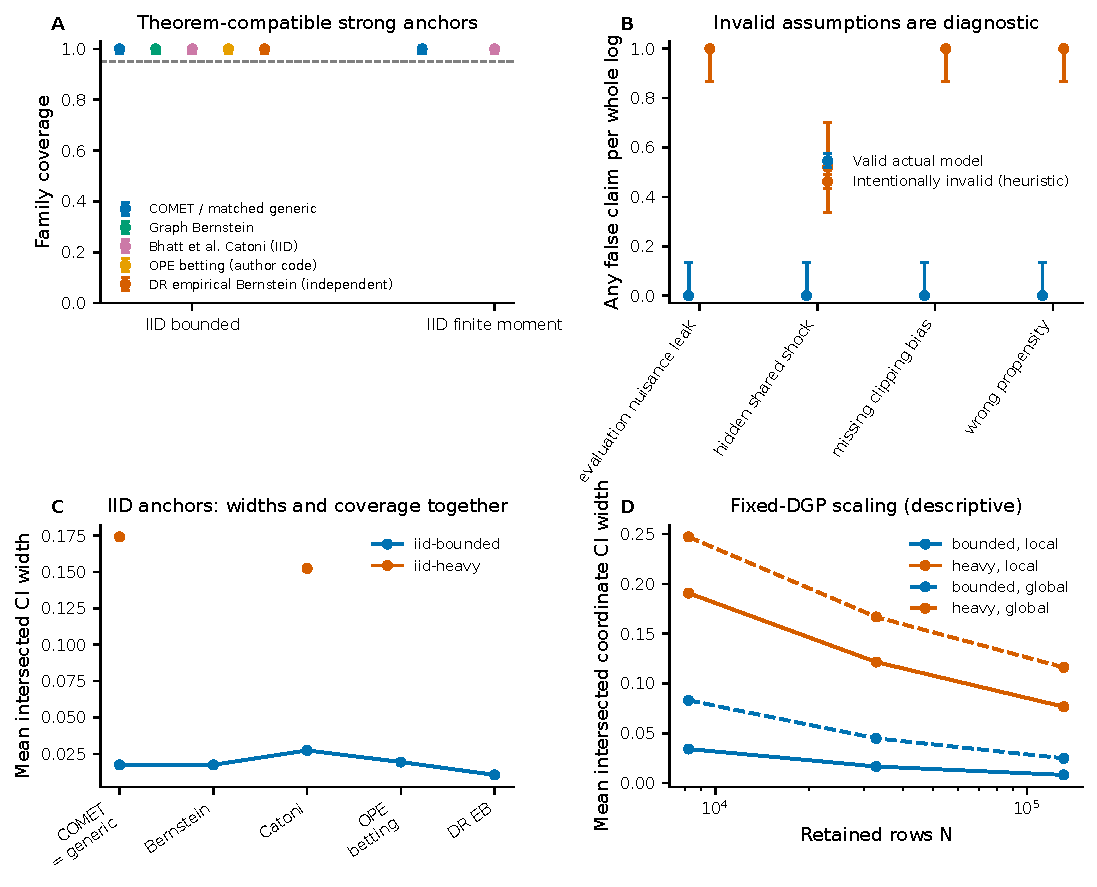
\includegraphics[width=\linewidth]{figures/supplementary_server_v2_v1/appendix_anchors_controls.pdf}
\caption{Supplementary evidence. Anchor coverage and negative-control false
claims have pointwise whole-log Wilson 95\% intervals. Widths are intersected
interval widths, not empirical moment estimates. The independent/bounded
comparators appear only where eligible; honest refusals have no error rate
and are omitted from that panel. Every fixed cell and both levels remain in
the accompanying exports, including the secondary betting coverage miss.}
\label{fig:post-supplementary}
\end{figure}

\clearpage
\section{Preserved historical confirmation}
\label{app:post-historical}

The preserved C-STAT study contains 6,000 independent complete logs, 1,000
in each of six fixed-design cells, with 1,134,000 candidate records. Its
seventeen eligible primary comparisons each covered 1,000 of 1,000 complete
families. Each fixed comparison has Wilson 95\% interval $[.996173,1]$;
this is a marginal Monte Carlo interval, not a simultaneous bound across all
seventeen comparisons and not a proof of validity. Methods share logs.
The twelve historical preflight logs are excluded.

\begin{table}[ht]
\centering
\caption{Preserved E0 results at 95\%, from the completed frozen report.
Widths are intersected with the known mean-class target range and divided by
its diameter. Nontriviality and no-decision rates are candidate descriptions,
not independent-log power. The original MOM has width ratio 1 everywhere.}
\label{tab:post-E0}
\small
\begin{tabular}{lrrrr}
\toprule
Cell & Exact MOM width & Graph width & Graph nontrivial & Graph no decision\\
\midrule
A & .872872 & .098821 & 100\% & 98.8\%\\
B & .916332 & .268917 & 100\% & 50.99375\%\\
C & 1 & .531225 & 100\% & 99.98125\%\\
D & 1 & .865982 & 61.80625\% & 93.79375\%\\
E & 1 & 1 & 31.24375\% & 100\%\\
F & 1 & N/A & N/A & N/A\\
\bottomrule
\end{tabular}
\end{table}

The graph method detected at least one true violation in 12, 1,000, 3, 0 and
0 of 1,000 independent logs in A--E respectively. Its 70\% detection fraction
among true-violating candidates in B is a different endpoint. Both MOM
methods in F were fully vacuous and always abstained; the bounded graph method
was inapplicable to F. These results describe the historical independent-block
model and do not validate the new heterogeneous connected-graph implementation.

The analytic A comparison in Equation~\eqref{eq:post-A-fixture} also shows why
the historical Chebyshev method's low detection is not an information limit.
Using the actual bounded residual range gives an eligible Hoeffding radius
small enough to guarantee detection on its coverage event. No historical
data were regenerated for this calculation and no new comparison was inserted
into the original confirmation family.


\end{document}
